\documentclass[a4paper,11pt,titlepage]{article}[11.3.2016]

\usepackage[slovak]{babel}
\usepackage[left=1.5cm,text={18cm, 25cm},top=2.5cm]{geometry}
\usepackage[utf8]{inputenc}
\usepackage{times}
\usepackage{amsthm}
\usepackage{amsmath,amsfonts,amssymb}
\usepackage{graphicx}
\usepackage{rotating}

\begin{document}
\begin{titlepage}
	\begin{center}
		{\Huge\textsc{Fakulta informačních technologií\\
		Vysoké učení technické v~Brně}}\\
		\vspace{\stretch{0.382}}    
	    {\LARGE{Dokumentácia projektu do predmetu \textit{Databázové systémy}\\
		 \vspace{5mm}
		 \Huge\textbf{{Hotel}}}}
		\vspace{\stretch{0.618}}
	\end{center}
	{\Large \hfill Dávid Bolvanský (xbolva00)\\
	\today \hfill Adrián Tóth (xtotha01)}
\end{titlepage}

\section*{Zadanie} 
Navrhnite IS hotela, ktorý by poskytoval prehľad o~dostupnosti izieb, údaje o~hosťoch, ich pobytoch v~hoteli, požiadav\-kách na služby, platby za izby, atď. Zákazníci môžu robiť rezervácie izieb (tým pádom musí zadať svoje osobné údaje). Klient si môže v~rámci jednej rezervácie objednať viac izieb, napríklad aj na iný dátum. Hoteli stačí mať informácie iba o~jednom klientovi, ktorý zastrešuje celý pobyt v~hoteli (o~ostatných účastníkoch pobyte nemusia byť dostupné žiadne informácie). Pobyt môže byť vytvorený na základe rezervácie, alebo k~rezervácii izby vôbec nemusí dôjsť, ak klient príde priamo na recepcii hotela. Jednotlivé typy izieb majú rôzne ceny, cena izby sa navyše môže líšiť podľa obdobia (turistická sezóna), na ktoré si klient izbu objednáva. Cena izby sa zároveň odvíja od toho, či si hosť izbu rezervuje dopredu, alebo až na mieste. Klient si môže priobjednať k~danému pobytu služby v~hoteli naviac, ako napr. prenájom bazéna, a to aj viackrát. IS ďalej bude schopný evidovať skutočne absolvované pobyty \,--\, tj. ktoré izby klient od kedy do kedy obýval a aké služby skutočne využil (od x do x na ktorej izbe). Pri každom pobyte je evidované, ktorý zamestnanec prevzal platbu za pobyt.

\section*{Doplnenie zadania} 
V~hoteli pracujú trvalí zamestnanci, ktorí sú zamestnaní na dobu neurčitú a o~ktorých je potrebné uchovávať údaj o~dátume prijatia do zamestnania v~hoteli, a zároveň tu pracujú aj zamestnanci, ktorí sú zamestnaní na dobu určitú a v~IS si uchovávame údaj o~ich pracovnej zmluve (od \,--\, do).

\newpage

\section{Generalizácia / špecializácia} 
Generalizáciu / špecializáciu sme v našom zadaní využili u zamestnanca hotela. Zamestnanec može byť buď trvalo zamestnaný, alebo môže byť zamestnaný na dobu určitú. 

\begin{center}
\begin{figure}[h]
    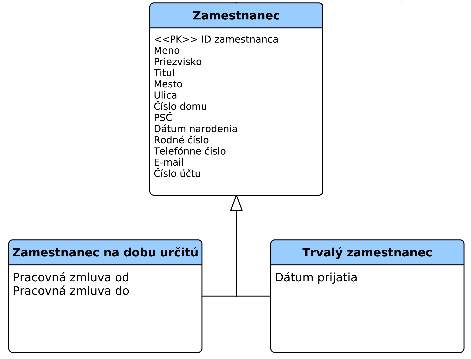
\includegraphics{generalizacia.png}
\end{figure}
\end{center}

\newpage

Pri transformácii tejto generalizácie/špecializácie sme vytvorili ďalšie dve tabuľky, a to ako pre trvale zamestnaného, tak aj pre dočasne zamestnaného zamestnanca hotela.

\begin{center}
\begin{figure}[h]
    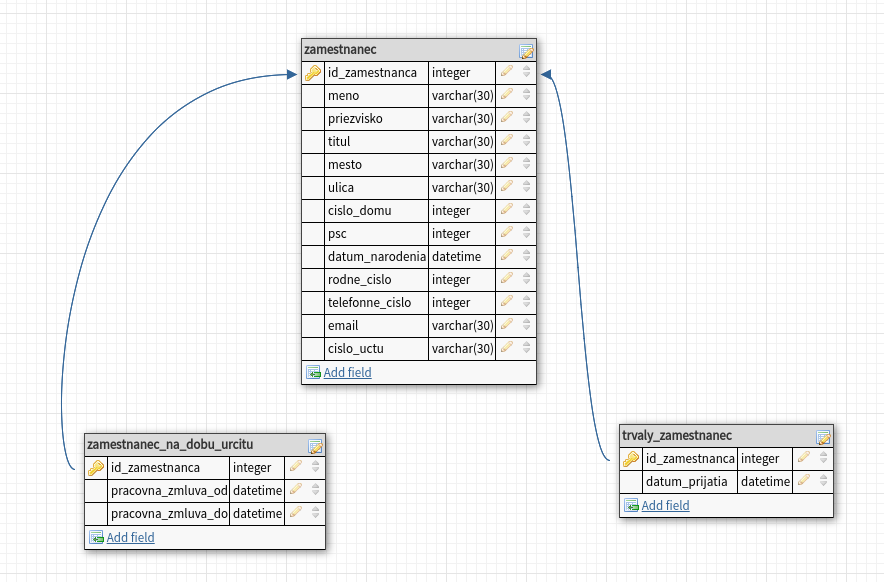
\includegraphics[scale=0.55]{generalizacia_tabulky.png}
\end{figure}
\end{center}

\section{Schéma relačnej databázy}
Nasledovná schéma popisuje finálnu schému relačnej databázy:

\begin{sidewaysfigure}
    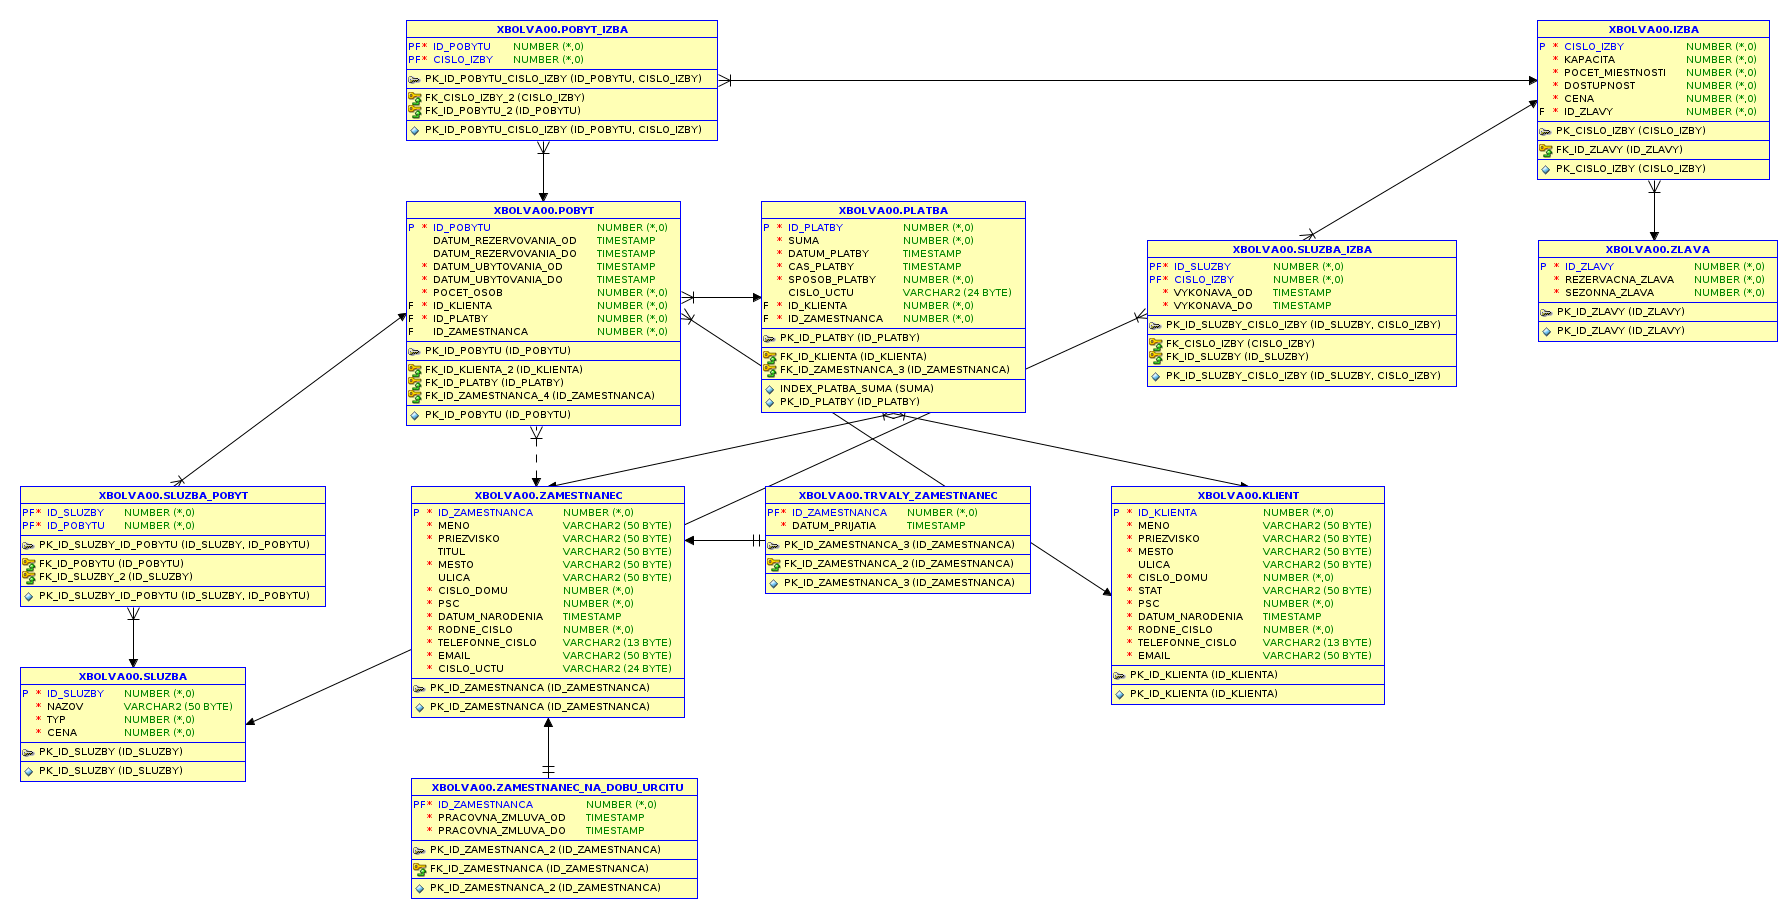
\includegraphics[scale=0.4]{finaldb.png}
\end{sidewaysfigure}

\newpage

\section{SQL skript}
Skript na začiatku vyčistí všetky databázové objekty pomocou \textit{DROP} na zabránie potenciálnym konfliktom. Následne sa vytvoria jednotlivé tabuľky, nastavia sa cudzie a primárne kľúče. Tabuľky sa potom naplnia dátami. Skript obsahuje niekoľko \textit{SELECT} príkazov, ktoré pokrývajú požiadavky určené zadaním projektu. Taktiež skript obsahuje triggery, procedúry, materializovaný pohľad, použitie indexu s \textit{EXPLAIN PLAN} a pridelenie prístupových práv druhému členovi tímu. Na potreby ladenia skriptu je v skripte zapnutý výstup servera.

\section{Triggery}
V rámci projektu sme implementovali tri databázové triggery. Prvým triggerom vyplývajúcim explicitne zo zadania projektu bol trigger na automatické generovanie hodnôt primárneho kľúča -- \textit{auto\_inkrementacia\_cisla\_izby}. V našom prípade sme tento trigger použili s tabuľkou \textit{IZBA}. Trigger sa realizoval pomocou sekvencie kvôli uchovaniu posledného čísla použitého ako hodnota primárneho kľúča. Sekvencia začína od čísla $200$ a inkrementuje sa po $1$.\\
\\
Ďalší trigger kontroluje správnosť rodného čísla klienta -- \textit{kontrola\_rodneho\_cisla\_klienta}. Trigger overuje počet číslic a správnosť dátumu v rodnom čísle. Ďalej rodné číslo musí byť deliteľné číslom $11$, na túto kontrolu sme použili funkciu \textit{MOD} na výpočet modula, zvyšku po delení. Taktiež sa kontroluje u rodného čísla s počtom číslic $9$, či neobsahuje neprípustnú koncovku $000$.\\
\\
Tretí trigger je automaticky prevádza sumu platby za pobyt z českých korún na eurá (uvažuje sa kurz $27$ pre jednoduchosť) -- \textit{prevod\_na\_eura}. Všetky tieto triggery majú príznak \textit{BEFORE INSERT ON}, čo znamená, že sa spúšťajú pred vložením dát do určitej tabuľky.

\section{Procedúry}
Súčasťou skriptu sú aj tri procedúry. Všetky procedúry obsahujú v sebe použitie kurzora a v každej procedúre bola použitá premenná s dátovým typom odkazujúcim sa na riadok či typ stĺpca tabuľky (\textit{table\_name.column\_name\%TYPE} alebo \textit{table\_name\%ROWTYPE}). Prvá procedúra výtvara štatistiku o zastúpení klientov z istého mesta v porovnaní s celou klientelou hotela -- \textit{zastupenie\_mesta\_v\_klientele}.
Procedúra má jeden parameter a ním je práve názov mesta. Súčasťou výpisu je celkový počet klientov, počet klientov z daného mesta a počet klientov z tohto mesta v pomere s celkovým počtom klientov. Tento pomer je vyjadrený v percentách. V procedúre je ošetrený stav delenia nulou, čo v tomto našom prípade znamená, že hotel nemá žiadnych klientov a tento fakt sa pri dosiahnutí výnimky vypíše na výstup. Pri ostatných chybách je vypísané chybové hlásenie s kódom $-20005$.\\
\\
Ďalšia procedúra kontroluje správnosť formátu emailovej adresy zamestnancov -- \textit{kontrola\_emailov\_zamestnancov}. Ak tento formát nespĺňa formát \textit{meno@domena}, na výstup je výpisané meno a priezvisko zamestnanca s chybne zadanou emailovou adresou. Ak dôjde k výnimke, je vypísané chybové hlásenie s kódom $-20006$.\\
\\
Posledná procedúra informuje o počte voľných izieb vzhľadom na ich kapacity -- \textit{volne\_izby\_podla\_kapacity}. Pre zjednodušenie uvažujeme, že hotel má izby s kapacitou od $1$ po $4$. Na výstupe sú informácie, koľko je voľných izieb na hoteli pre jednotlivé kapacity. Chybové hlásenie s kódom $-20007$ je vypísané v prípade chyby/výnimky počas analýzy dát v tabuľkách.

\newpage

\section{Materializovaný pohľad}
Našou úlohou bolo implementovať materializovaný pohľad patriaci druhému členovi tímu, ktorý používa tabuľky prvého člena tímu pomocou zápisu \textit{login.table}. Bolo potrebné vytvoriť materializované záznamy (logy) obsahujúce zmeny hlavnej tabuľky, ktoré služia na to, aby bolo možné používať rýchlu obnovu po potvrdení zmien namiesto kompletnej obnovy, ktorá by vyžadovala spúštať celý dotaz materializovaného pohľadu, čo by trvalo dlhšie. Následne sme vytvorili samotný materializovaný pohľad, ktorý sa týkal \textit{SELECT} dotazu s prirodzeným spojením tabuliek \textit{POBYT} a \textit{KLIENT} a slúžil na výpis rodného čísla klienta, a dátumov odkedy a dokedy je ubytovaný na hoteli.\\ 
\\
Nastavili sme nasledovné možnosti materializovaného pohľadu:\\
\noindent
\textit{CACHE} -- optimalizácia čítania z pohľadu\\
\textit{BUILD IMMEDIATE} -- naplnenie pohľadu po jeho vytvorení\\
\textit{REFRESH FAST ON COMMIT} -- aktualizácia pohľadov podla záznamov po potvrdení zmien v tabulkách\\
\textit{ENABLE QUERY REWRITE} -- použitie materializovaného pohľadu optimalizátorom\\
\\
Pomocou \textit{EXPLAIN PLAN} sme požiadali o vysvetlenie dotazu, čím sme získali prehľad o operáciach vykonávaných počas dotazu obsahujúceho prirodzené spojenie týchto tabuliek. 

\begin{center}
\begin{figure}[h]
    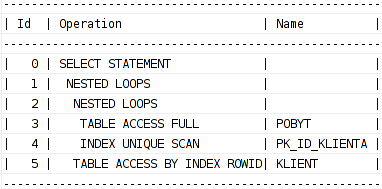
\includegraphics{nomatview.png}
\end{figure}
\end{center}

\noindent
Povolili sme možnosť \textit{QUERY REWRITE} pre optimalizátor pomocou \textit{ALTER SESSION SET query\_rewrite\_enabled = TRUE} a znovu sme použili EXPLAIN PLAN na získanie prehľadu o operáciach v dotaze. V tomto získanom prehľade je možné vidieť, že došlo k použitiu materializovaného pohľadu. Optimalizátor bude používať materializovaný pohľad pri vyhodnocovaní dotazu, na ktorom je tento pohľad založený.

\begin{center}
\begin{figure}[h]
    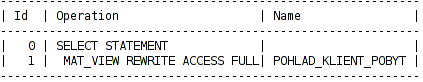
\includegraphics{matview.png}
\end{figure}
\end{center}

\newpage

\section{\textit{EXPLAIN PLAN} a vytvorenie indexu}
\textit{EXPLAIN PLAN} nám slúži na vysvetlenie dotazu databázou, čiže získame plán ako databáza spracováva daný dotaz. \textit{EXPLAIN PLAN} sme použili na \textit{SELECT} dotaz, ktorým získame meno, priezvisko, rodné číslo a počet súm platieb jednotlivých klientov, kde platí, že suma platby za pobyt bola v rozmedzí od $1000$ do $1500$ českých korún.\\
\\
\textit{EXPLAIN PLAN} pre tento dotaz bez využitia indexu vyzerá nasledovne:
\begin{center}
\begin{figure}[h]
    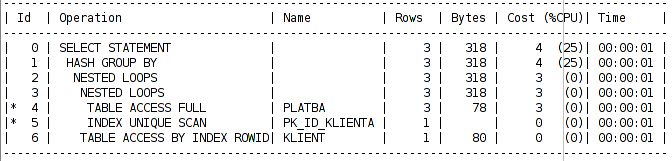
\includegraphics[scale=0.7]{pred.png}
\end{figure}
\end{center}

\noindent
Rozbor tohto získaného plánu:\\
\textit{SELECT STATEMENT} znamená, že sa uskutočnil \textit{SELECT} dotaz. \textit{HASH GROUP BY} značí zoskupovanie položiek podľa hashovacieho kľúča. Ďalej máme dvakrát \textit{NESTED LOOPS}, čo reprezentuje samotné spojenie, kde pre každú položku prvej tabuľky sa prejdú všetky riadky z druhej tabuľky. Nasleduje \textit{TABLE ACCESS FULL}, čo značí prechod celou tabuľkou od začiatku bez použitia indexov. \textit{TABLE UNIQUE SCAN} reprezentuje prístup k tabuľkám cez \mbox{B--strom}, kde získame jeden jedinečný riadok podla primárneho kľúča v tabuľke \textit{KLIENT}.\\

\noindent
Následne sme vytvorili index pomocou \textit{CREATE INDEX index\_platba\_suma ON platba(suma)} a znovu spustili \textit{EXPLAIN PLAN}:

\begin{center}
\begin{figure}[h]
    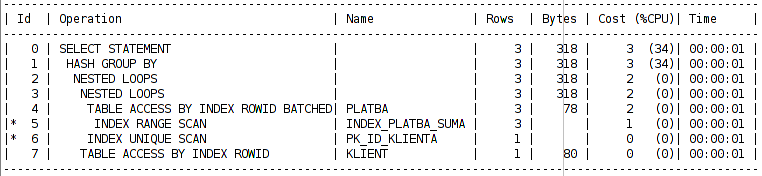
\includegraphics[scale=0.7]{po.png}
\end{figure}
\end{center}

\noindent
Ako je možné vidieť z výsledného plánu po použití indexu, cena (cost) sa znížila. Plán s použití indexu obsahuje informáciu, že na tabuľke \textit{PLATBA} sa vykonával \textit{TABLE ACCCES BY INDEX ROWID BATCHED}, kedy sa pristupuje do tabuľky cez konkrétny riadok, čo znamená, že databáza použila náš index.

\section{Pridelenie prístupových práv}
Druhý člen tímu má pridelené práva na úrovni bežného zamestnanca. Znamená to, že nemá práva na úpravu tabuliek s dátami o zamestnancoch, službách a zľavách. Taktiež nemôže použiť procedúru na kontrolu emailov jednotlivých zamestnancov. K ostatným tabuľkám, ako sú napríklad tabuľky s platbami, pobytmi, klientami a izbami, má zamestnanec plný prístup a taktiež môže používať zvyšné dve procedúry.
Pridelenie prístupových práv k tabuľkám je realizované pomocou \textit{GRANT ALL ON [table] TO [user]}, k materializovanému pohľadu pomocou \textit{GRANT ALL ON [materialized view] TO [user]} a k procedúram pomocou \textit{GRANT EXECUTE ON [procedure] TO [user]}. Druhý člen tímu sa pripojí k databáze prvého člena tímu pomocou \textit{ALTER SESSION SET CURRENT\_SCHEMA = [schema name]}, kde \textit{schema name} je prihlasovacie meno prvého člena tímu. 

\section{Zhodnotenie}

Skript sme vypracovali v nástroji \textit{SQL Developer}, v prostredí \textit{Oracle} na školskom serveri \textit{Oracle 12c}. Informácie na vypracovanie projektu sme čerpali z materiálov k predmetu \textit{IDS}, kladne hodnotíme aj demonštračné cvičenia, ktoré nám viac ozrejmili jednotlivé časti projektu. Čerpali sme aj z oficiálnej \textit{Oracle} dokumentácie a preštudovali sme si súvisiace články na internete k našej problematike.

\end{document}